\documentclass[a4paper,11pt]{article}

\usepackage[margin=2.5cm]{geometry}
\usepackage{amsmath,amssymb,amsthm,amsfonts}
\usepackage{enumerate}
\usepackage{mathabx}
\usepackage{braket}
\usepackage[framemethod=tikz]{mdframed}
\usepackage{dsfont}
\usepackage{listings}
\usepackage{color}
\definecolor{dkgreen}{rgb}{0,0.6,0}
\definecolor{gray}{rgb}{0.5,0.5,0.5}
\definecolor{mauve}{rgb}{0.58,0,0.82}
\usepackage{fancyhdr}
\usepackage{graphicx}
\usepackage{epstopdf}
\usepackage{pgfplots}
\usepackage{tikz}
\usepackage{pgfplots}

\lstset{frame=tb,
	language=C++,
	aboveskip=3mm,
	belowskip=3mm,
	showstringspaces=false,
	columns=flexible,
	basicstyle={\small\ttfamily},
	numbers=none,
	numberstyle=\tiny\color{gray},
	keywordstyle=\color{blue},
	commentstyle=\color{dkgreen},
	stringstyle=\color{mauve},
	breaklines=true,
	breakatwhitespace=true,
	tabsize=3
}

\newtheorem*{remark}{Remark}

\newtheoremstyle{break}
{\topsep}{\topsep}%
{\itshape}{}%
{\bfseries}{}%
{\newline}{}%
\theoremstyle{break}

\newtheoremstyle{break2}
{\topsep}{\topsep}%
{}{}%
{\bfseries}{}%
{\newline}{}%
\theoremstyle{break2}

\theoremstyle{break}
\newtheorem{theorem}{Theorem}[section]
\newtheorem{proposition}[theorem]{Proposition}
\newtheorem{corollary}[theorem]{Corollary}
\newtheorem{lemma}[theorem]{Lemma}

\theoremstyle{break2}
\newtheorem{definition}[theorem]{Definition}
\newtheorem{example}[theorem]{Example}

\newcommand{\R}{\mathbb{R}}
\newcommand{\N}{\mathbb{N}}
\newcommand{\Z}{\mathbb{Z}}
\newcommand{\Q}{\mathbb{Q}}
\newcommand{\C}{\mathbb{C}}
\newcommand{\F}{\mathbb{F}}
\newcommand{\K}{\mathbb{K}}
\newcommand{\lP}{\mathbb{P}}
\newcommand{\lS}{\mathbb{S}}
\newcommand{\cA}{\mathcal{A}}
\newcommand{\cB}{\mathcal{B}}
\newcommand{\cL}{\mathcal{L}}
\newcommand{\cF}{\mathcal{F}}
\newcommand{\cO}{\mathcal{O}}
\newcommand{\cM}{\mathcal{M}}
\newcommand{\cC}{\mathcal{C}}
\newcommand{\cE}{\mathcal{E}}
\newcommand{\cP}{\mathcal{P}}
\newcommand{\s}{\sigma}
\newcommand{\e}{\varepsilon}
\newcommand{\Cyl}{\textnormal{Cyl}}
\newcommand{\de}{\textnormal{ d}}
\newcommand{\I}{\mathds{1}}
\newcommand{\wto}{\rightharpoonup}

\title{C1 - Assignment 2 Report}
\author{Student Number: u1858921}
\date{Submission Deadline: 6pm November 21st, 2018}

\begin{document}
	\maketitle
	\tableofcontents
	
\section{Introduction}
In this report we study numerical solutions to boundary value problems, in particular for the advection-reaction-diffusion equation under given boundary conditions. In general, we define a boundary value problem as follows
\begin{mdframed}[]
	Let $ \Omega \subseteq \R^d $, $ d = 1,2 $, be a bounded simply connected open domain. Find, for $ f,v $ given, a function $ u $ such that
	\begin{align*}
	\cL[u] = f, \quad \text{in } \Omega,\qquad u = v,  \quad \text{on } \partial\Omega,
	\end{align*}
	where $ \cL = -\Delta u + \mathbf{p}\cdot\nabla u + qu $, with $ \mathbf{p},q $ given smooth, bounded functions.
\end{mdframed}
In this report, we deal with a \emph{Dirichlet problem}, in which we ask to find the solution of the equation in the interior of $ \Omega $ while prescribing its value on the boundary $ \partial\Omega $.\\\\
We obtain numerical solutions of the advection-reaction-diffusion equation through the \emph{finite-difference} (FD) method. The approach of the FD method is to evaluate the given operator $ \cL $ at a set of discretisation points $ (x_j)_{j=1}^J $ with the derivatives within replaced by difference quotients of the approximated solution, $ U $. These difference quotients (e.g. $ \partial^-, \partial^+, \partial^+\partial^- $) are obtained by truncating the Taylor expansion of the exact solution about the discretisation points $ x_j $. Then after this discretisation, one should obtain a system of equations, which can be rewritten as a linear matrix problem, i.e. $ A\mathbf{U}=\mathbf{f} $ for the approximate solution $ \mathbf{U} $ and given data $ \mathbf{f} $. There are a number of ways in which linear problems can be solved, on that we shall use is the \emph{Gauss-Seidel} method discussed in Assigment 1 of this course.\\\\
In section 2 we go through the discretisation of the advection-reaction-diffusion equation throgh the finite difference method and present its numerical implementation. In section 3, we test the numerical scheme obtained in section 2 on the advection-diffusion-reaction equation with known analytical solutions as to deduce the error of the scheme and some analyical results. In section 4, we provide a conclusion to the analysis performed in the previous sections.
\section{Problem}
The aim of this report is to numerically deduce (throught the method of finite differences) the solutions of the advection-diffusion-reaction equation
\begin{align*}
-\alpha u'' + \beta u' + \gamma u = 0,
\end{align*}
for given parameter values $ \alpha,\beta $ and $ \gamma $. In particular, we seek to find the the solutions of the linear advection diffusion equation
\begin{align}\label{Eq:LAD}
-\alpha u'' + \beta u' = 0, \quad u(0) = 0,\ u(L) = 1,
\end{align}
and the linear diffusion reaction equation
\begin{align}\label{Eq:LDR}
-\alpha u'' + \gamma u = 0, \quad u(0) = 0,\ u(L) = 1,
\end{align}
in the domain $ \Omega = [0,1] $. For equation \eqref{Eq:LAD}, define the so-called \emph{P\'{e}clet} number, $ Pe $, through
\begin{align*}
Pe = \frac{|\beta|L}{2\alpha},
\end{align*}
and for the equation \eqref{Eq:LDR}, the so-called Damk\"{o}hler number
\begin{align*}
Da = \frac{\gamma}{\alpha}.
\end{align*}

\subsection{Discretisation Through Finite-Differences}
We begin by discretising the general boundary value problem
\begin{align}\label{Eq:GeneralADR}
-\alpha u'' + \beta u' + \gamma u = 0, \quad u(0) = 0,\ u(L) = 1.
\end{align}
When we require equation \eqref{Eq:LAD} or \eqref{Eq:LDR}, we choose $ \gamma = 0 $ or $ \beta = 0 $ respectively. We discretise equation \eqref{Eq:GeneralADR} by finite differences with simple centred schemes for second and first order derivatives. We begin by letting $ (x_j)_{j=0}^{J+1} $ be a partition of the interval $ \Omega = [0,L] $ such that $ 0 = x_0 < x_1 < x_2 < \cdots < x_J < x_{J+1} = L $. We denote the $ j $th interval by $ I_j = [x_{j-1},x_j] $ with the mesh size $ h_j = |I_j| $. Within this report, we consider a uniform mesh size, and therefore set $ h := h_j $ for all $ j $, hence $ x_j = jh $.
\begin{figure}[h]
	\centering
	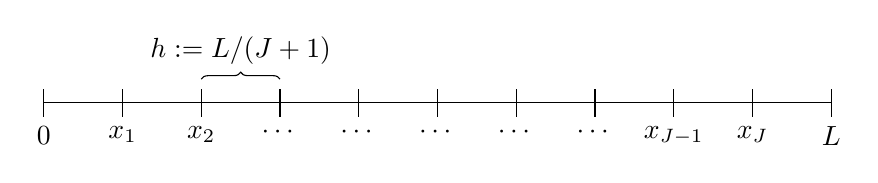
\begin{tikzpicture}
	\draw(0,0)--(10,0);
	\foreach \x/\xtext in {0/$0$,1/$ x_1 $,2/$ x_2 $,3/$ \cdots $,4/$ \cdots $,5/$ \cdots $,6/$ \cdots $,7/$ \cdots $,8/$ x_{J-1} $,9/$ x_J $,10/$L$}
	\draw(\x,5pt)--(\x,-5pt) node[below] {\xtext};
	\draw[decorate, decoration={brace}, yshift=2ex]  (2,0) -- node[above=0.4ex] {$ h := L / (J+1) $}  (3,0);
	\end{tikzpicture}
\end{figure}
Now let $ U_j := u(x_j) $ for each $ j \in \{1,\ldots,J\} $ and define $ \mathbf{U} = (U_1,\ldots,U_J) $, which denotes the approximation of $ u $ on the interior of the partitioning of $ [0,L] $. Then the discrete problem approximating the continuous problem \eqref{Eq:GeneralADR} is given by 
\begin{align}\label{Eq:FDD}
-\alpha\partial^-\partial^+ U_j + \beta \partial^0U_j + \gamma U_j = 0, 
\end{align}
for $ j = 1,\ldots,J $ with $ U_0 = u(0) = 0 $ and $ U_{J+1} = u(L) = 1 $, where
\begin{align*}
\partial^-\partial^+U_j = \frac{U_{j-1} - 2U_j + U_{j+1}}{h^2},\quad \partial^0 = \frac{U_{j+1} - U_{j-1}}{2h}.
\end{align*}
Equation \eqref{Eq:FDD} can be rewritten as
\begin{align*}
\left(-\frac{\alpha}{h^2} - \frac{\beta}{2h}\right)U_{j-1} + \left(\frac{2\alpha}{h^2} + \gamma\right)U_j + \left(-\frac{\alpha}{h^2} + \frac{\beta}{2h}\right) = 0,
\end{align*}
for $ j = 1, \ldots, J $, which gives rise to the following linear equation
\begin{align}\label{Eq:LinearSystem}
A\mathbf{U} = \mathbf{f},
\end{align}
where $ A = (a_{ij}) \in \R^{J \times J} $ is such that
\begin{align*}
a_{ij} =
\begin{cases}
-\frac{\alpha}{h^2} - \frac{\beta}{2h} & \text{if } j = i-1, \\
\frac{2\alpha}{h^2} + \gamma & \text{if } j = i, \\
-\frac{\alpha}{h^2} + \frac{\beta}{2h} & \text{if } j = i+1,
\end{cases}
\end{align*}
and $ \mathbf{f} = (f_i) \in \R^{J} $ is such that 
\begin{align*}
f_i =
\begin{cases}
0 & i \neq J, \\
\frac{\alpha}{h^2} - \frac{\beta}{2h} & i = J.
\end{cases}
\end{align*}
We make note of the fact that the matrix $ A $ is sparse and tridiagonal. This completes the finite difference discretisation, and we may now apply numerical inversion techniques to the matrix $ A $ to deduce the numerical solution, $ \mathbf{U} $, of the problem \eqref{Eq:GeneralADR}. If $ A $ is made diagonally dominant, then we may use the Gauss-Seidel numerical scheme implemented in Assignment 1 to solve the linear system. 

\subsection{Numerical Implementation}
To implement the above discretisation into a numerical scheme, we begin by creating a class called \texttt{FiniteDifference} shown below.

\begin{lstlisting}
class FiniteDifference
{
public:
	FiniteDifference(); // Default Constructor
	FiniteDifference(int J, double L, double alpha, double beta, double gamma, double b_0, double b_L);
	FiniteDifference(const FiniteDifference& scheme); // Copy Constructor
	~FiniteDifference(); // Destructor

	int getJ();
	double getL();
	double getAlpha();
	double getBeta();
	double getGamma();
	double getb_0();
	double getb_L();

	SparseMatrix constructMatrix(); // Constructs the "differential operator" matrix A

private:
	int J_; // The number of points in the discretisation
	double L_; // Length of interval
	double b_0_, b_L_; // Boundary conditions
	double alpha_, beta_, gamma_; // Equation parameters
};
\end{lstlisting}
To carry out the finite difference method described above, we define the member function \texttt{constructMatrix} of the class \texttt{FiniteDifference} to constuct the matrix $ A $ define in equation \eqref{Eq:LinearSystem}.
\begin{lstlisting}
SparseMatrix FiniteDifference::constructMatrix()
{
	double h = L_/(double) (J_ + 1); // Setting the mesh size
	SparseMatrix A = SparseMatrix(J_,J_);
	double D = 2*alpha_/(double) (h*h) + gamma_; // Diagonal terms of A
	double UD = -(alpha_ - h*beta_/2.0)/(double) (h*h); // Upper-diagonal terms of A
	double LD = -(alpha_ + h*beta_/2.0)/(double) (h*h); // Lower-diagonal terms of A
	for (int i = 0; i < J_; ++i)
	{
		for (int j = 0; j < J_; ++j)
		{
			if(j == i + 1) // Upper-diagonal entries
			{
				A.addEntry(i, j, UD);
			}
			else if(j == i) // Diagonal entries
			{
				A.addEntry(i, j, D);
			}
			else if (j == i - 1) // Lower-diagonal entries
			{
			A.addEntry(i, j, LD);
			}
		}
	}
	return A;
}
\end{lstlisting} 
We then proceed to solve the linear system in equation \eqref{Eq:LinearSystem} by inverting it against $ \mathbf{f} $ using the Gauss-Seidel numerical scheme, described in the previous assignment, to obtain the approximate solution to the problem \eqref{Eq:GeneralADR} in the form of a STL vector $ \mathbf{U} $.
\section{Results}
We can test the finite-difference approximation by analysing the error (using the $ L^{\infty} $ norm) between the numerical and analytical solution. For this, we consider the cases of equations \eqref{Eq:LAD} and \eqref{Eq:LDR} separately.
\subsection{Linear Advection-Diffusion Equation}
We can in fact solve equation \eqref{Eq:LAD} analytically with the given boundary conditions to obtain a unique solution of the following form
\begin{align}\label{Eq:AnalyticalAD}
u(x) = \frac{1 - \exp\left(\frac{\beta x}{\alpha}\right)}{1 - \exp\left(\frac{\beta L}{\alpha}\right)}, \quad x \in [0,L],
\end{align}
for $ \alpha \neq 0 $ and $ \beta \in \R $. We note that as $ \beta = 0 $, $ u(x) = x $, which is the limiting behaviour of the solution \eqref{Eq:AnalyticalAD}.
To be able to use the Gauss-Seidel algorithm, we require that the discretisation matrix $ A $ is diagonally dominant. We can guarantee this as along as
\begin{align*}
\left|\frac{2\alpha}{h^2}\right| \geq \left|-\frac{\alpha}{h^2} - \frac{\beta}{2h}\right| + \left|-\frac{\alpha}{h^2} + \frac{\beta}{2h}\right| \geq \left|\frac{\beta}{h}\right|,
\end{align*}
that is $ 2|\alpha| > h|\beta| $. Since $ h := \frac{L}{J+1} $, where $ J $ denotes the number of discretisation points, it follows that
\begin{align*}
J+1 \geq \frac{|\beta|L}{|\alpha|} \geq Pe. 
\end{align*}
Thus if the number of disretisation points $ J $ is greater that the Pecl\'{e}t number minus one ($ J > Pe - 1 $), then we are guaranteed to have convergence of the approximate solution to the correct solution through the use of Gauss-Seidel. Taking this into account, along with knowing the analytical solution, we can deduce the error, $ \|u_h - u\|_{\infty} $, of the numerical solution with respect to the analytical solution for various different values of $ \alpha, \beta, \gamma $ and number of discritisation points $ J $. The error plots for this can be seen in Figure \ref{Fig:ErrorLAD}.
\begin{figure}[h!]
	\centering
	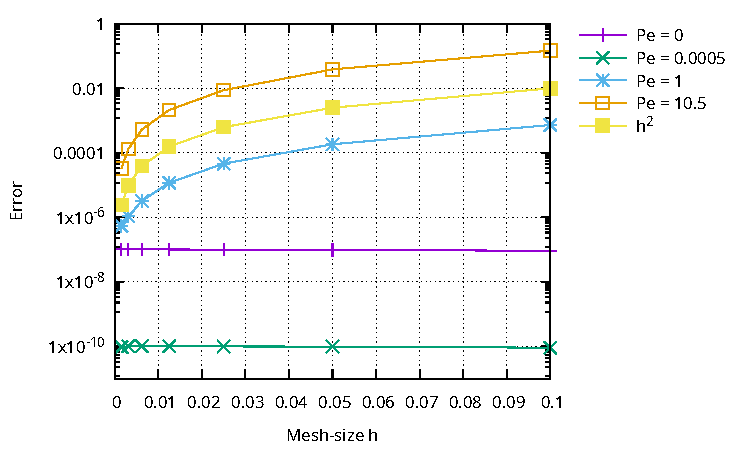
\includegraphics{Error_plots.pdf}
	\caption{Error between the analyical and numerical solution of equation \eqref{Eq:LAD} for variaous Pecl\'{e}t numbers $ Pe $ and discretisation points $ J $. \label{Fig:ErrorLAD}}
\end{figure}
\noindent
From Figure \ref{Fig:ErrorLAD}, we see that the error between the analytical solution and the numerical solution decreases exponentially for Peclet numbers of order at least 1, but when $ Pe = 0.0005 $, we observe that the error is very small and decreases extremely slowly as the number of points $ J $ increases. We know that by stability
\begin{align*}
\|r_hu - U\|_{\infty} \leq C \|\cL_h(r_h u) - \cL_h U \|_{\infty},
\end{align*}
for some constant $ C $. By Taylor expansion we know that
\begin{align*}
\|r_h u - u_h\|_{\infty} \leq \frac{h^2}{12}\|u^{(4)}\|_{\infty},\quad \|r_hu' - u_h'\|_{\infty} \leq \frac{h^2}{6}\|u^{(3)}\|_{\infty}.
\end{align*}
Therefore, we can obtain the following bound on the error
\begin{align*}
\|r_h u - u_h\|_{\infty} &\leq C\|-\alpha r_h u'' + \beta r_h u' + \alpha u_h'' - \beta u_h'\|_{\infty} \\
&\leq C\left(|\alpha|\|r_h u'' - u_h''\|_{\infty} + |\beta|\|r_h u' - u_h' \|_{\infty}\right) \\
&\leq C\left(\frac{|\alpha|h^2}{12}\|u^{(4)}\|_{\infty} + \frac{|\beta|h^2}{6}\|u^{(3)}\|_{\infty}\right).
\end{align*}
Since we know the analytical solution, for $ k = 3,4 $
\begin{align*}
u^{(k)}(x) =-\frac{\left(\frac{\beta}{\alpha}\right)^k}{1 - \exp\left(\frac{\beta L}{\alpha}\right)}\exp\left(\frac{\beta x}{\alpha}\right),
\end{align*}
therefore, for $ k = 3,4 $
\begin{align*}
\|u^{(k)}\|_{\infty} = \left|\frac{\beta}{\alpha}\right|^{k}\left|\frac{\exp\left(\frac{\beta L}{\alpha}\right)}{1 - \exp\left(\frac{\beta L}{\alpha}\right)}\right| =: g(\alpha,\beta).
\end{align*}
Then
\begin{align*}
\|r_hu - u_h\|_{\infty} \leq C\frac{h^2}{4}\frac{|\beta|^4}{|\alpha|^3}g(\alpha,\beta).
\end{align*}
Therefore, the order of convergence is at least of order $ 2 $, which was expected since that is the order of consistency.
\begin{figure}[h!]
	\centering
	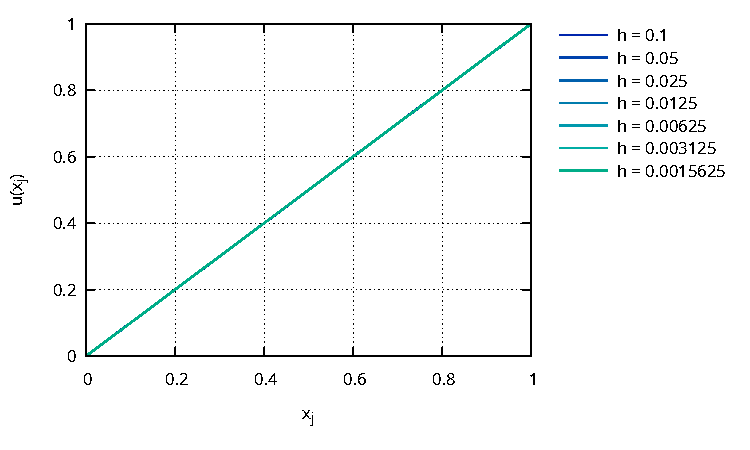
\includegraphics{Solution_plots_Pe_0.pdf}
\end{figure}
\begin{figure}[h!]
	\centering
	\includegraphics{{Solution_plots_Pe_0.0005}.pdf}
\end{figure}
\begin{figure}[h!]
	\centering
	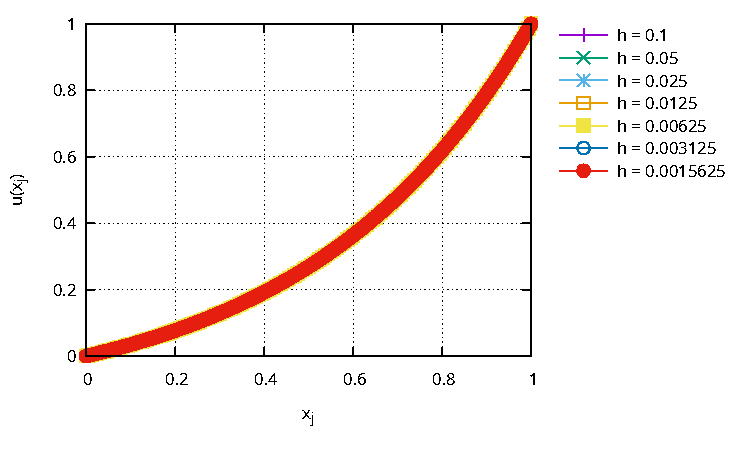
\includegraphics{Solution_plots_Pe_1.pdf}
\end{figure}
\begin{figure}[h!]
	\centering
	\includegraphics{{Solution_plots_Pe_10.5}.pdf}
\end{figure}
\subsection{Linear Diffusion-Reaction Equation}
We can also solve equation \eqref{Eq:LDR} analytically with the given boundary conditions to obtain a unique solution of the following form
\begin{align*}
u(x) = \frac{\sinh\left(\sqrt{\frac{\gamma}{\alpha}}x\right)}{\sinh\left(\sqrt{\frac{\gamma}{\alpha}}L\right)}, \quad x \in [0,L].
\end{align*}

\section{Conclusion}



\end{document}
